\subsection{LETs based on organic thin films}\label{sec:thinfilms} %Armin|Cees
The most appealing property of organic materials used for electronic and photonic applications, is that they can be deposited on many different type of surfaces such as a CMOS or cheap materials like plastic and glass. This, in turn, enables easy and cheap fabrication, which is of course an important driver for further developments. Organic materials can be produced with low-cost, large scale industrial production processes such as direct printing, ink-jet and other solution based techniques. Organic material thin film structures, which only require small amounts of material, are ideal for markets where low-cost production is of high importance, and performance does not require inorganic devices.

Also organic materials may be used to create multifunctional devices, using extremely simple device structures. OLETs represent a step towards this possibility. They combine electron and hole-effect transport, light emission and electron switching.

OLEDs enable electroluminescense in the same materials as OLETs, though with different driving schemes. The vertical structure of OLEDs enables low-voltage-driven light-emission, charge transport occurs perpendicular and through the plane of different layers. In OLETs charge transport occurs parallel and through the plane. An schematic representation is shown in figure \ref{fig:thinfilms}. This difference in configuration causes OLEDs to demonstrate bulk charge transport and OLETs to demonstrate field-effect charge transport. Another notable difference is the distance the minority carriers need to travel before recombining radiatively. In OLEDs the distance the charges travel are in the order tens of nanometres, for typical ambipolar OLETs the distance is in the order of hundreds of nanometres or more. This larger distance requires stricter charge transport properties of OLET materials.

\begin{figure}[!ht]
 \begin{center}
  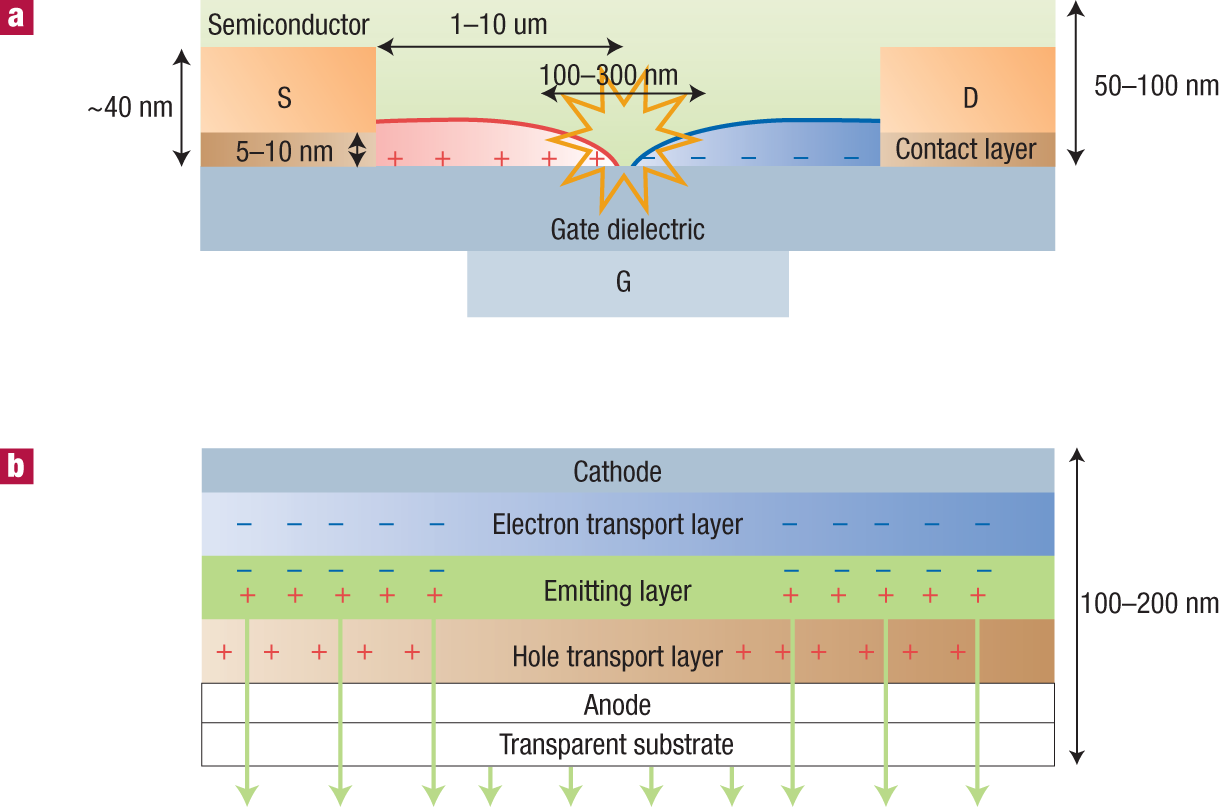
\includegraphics[width=0.8\textwidth]{fig_2}
  \caption{Schematic representation of OLET and OLED. (a) Horizontal charge transport in OLETs. (b) Vertical charge transport in OLEDs. Picture from \citet{Muccini}.}
  \label{fig:thinfilms}
 \end{center}
\end{figure}

For OLETs, the distance between the exciton formation region and the metal electrodes is much larger. Here for they are less affected by electron-metal quenching. This effect is further reduced by the availability of a third electrode that balances electron and hole currents. These structural advantages make OLETs more favourable for high-brightness electroluminescense and highly integrated devices. These advantages however do rely on the further development of organic materials.
